
\section{Model Fitting and Line and Circle Detection}
Edge detection is usually not enough as there are usually more than one line in an image and many edges that do not belong to a line.
There might be noise in the edges belonging to a line which brings them out of alignment. Lines might also not be complete.

\subsection{Model Fitting}
Model fitting is an algorithm that finds or fits a high-level explanation or model that explains the observations well.
In this case the edges are the observations and the model are one or more line.

\subsection{Voting Algorithms}
Voting algorithms are a general technique for decision methods.

\begin{enumerate}
	\item Every feature casts votes for all models that are compatible with it
	\item Choose models that accumulate a lot of votes
\end{enumerate}

Clutter and noise will cast a lot of votes, but are inconsistent. Instead, features belonging to a model will concentrate a lot of votes for that model.

\subsection{Hough Transform}
\begin{enumerate}
	\item Every \textbf{edge point} casts votes for \textbf{all lines that are compatible} with it
	\item Choose \textbf{lines} that accumulated a lot of votes
\end{enumerate}

\begin{figure}[H]
	\centering
	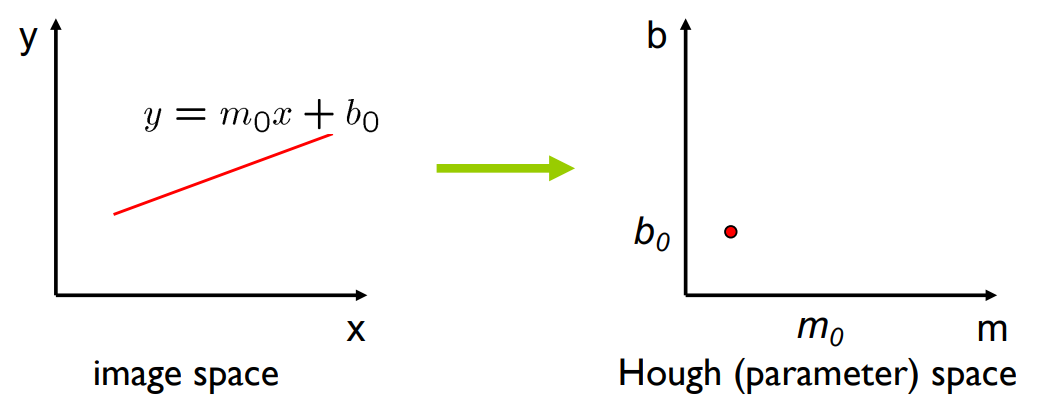
\includegraphics[width=0.8\linewidth,keepaspectratio]{img/line_representation_hough}
	\caption{Line representation in Hough space}
\end{figure}

\begin{figure}[H]
	\centering
	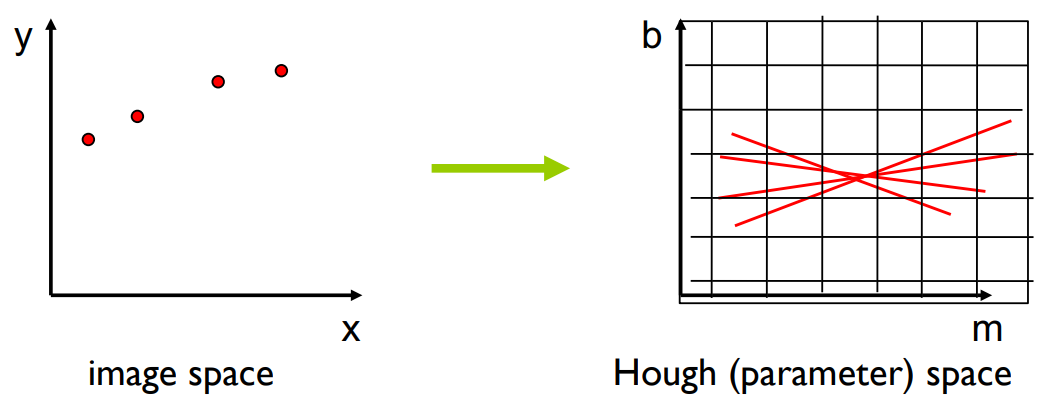
\includegraphics[width=0.8\linewidth]{img/points_representation_hough}
	\caption{Points on a line in normal space almost intersect in Hough space}
	\label{fig:pointsrepresentationhough}
\end{figure}

\noindent
The problem with this approach is that
\begin{enumerate}[label=\alph*.]
	\item the parameter space $(m,b)$ is \textbf{not bounded}
	\item \textbf{vertical lines} can not be represented
\end{enumerate}

\subsection{Representation of Lines in Polar Coordinates}

\begin{figure}[H]
	\centering
	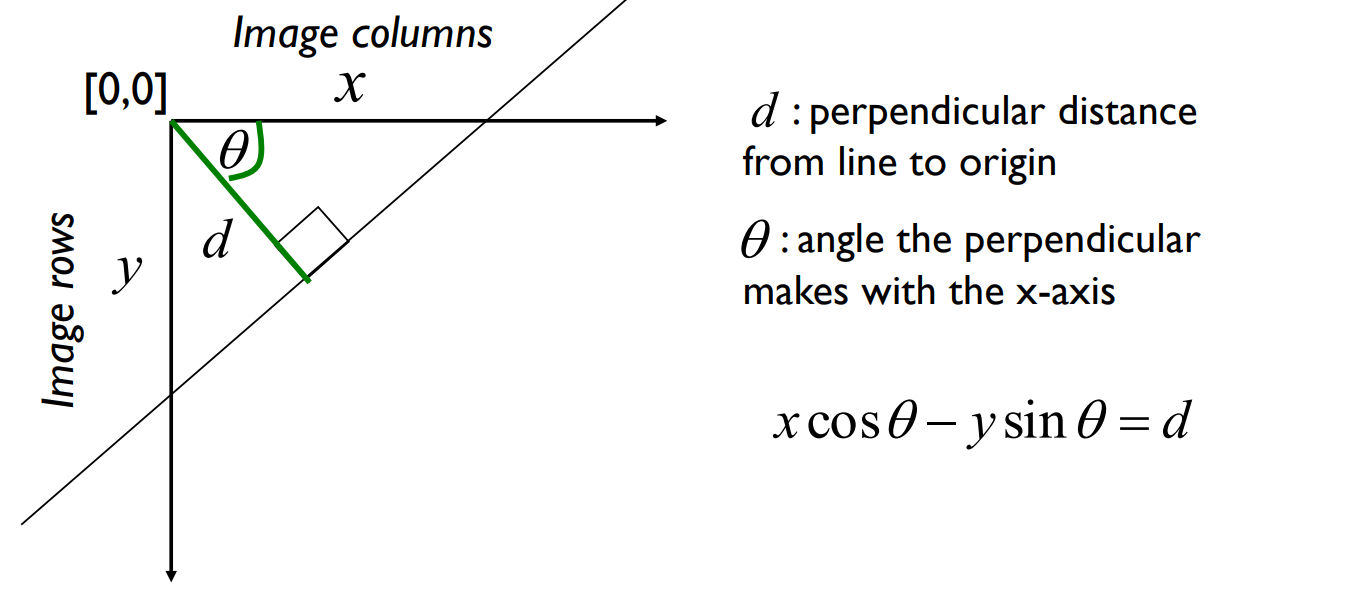
\includegraphics[width=0.8\linewidth]{img/line_representation_polar}
	\caption{Line representation with polar parameters}
	\label{fig:linerepresentationpolar}
\end{figure}

This approach solves both the problem of unboundedness and representation. The parameter $\theta$ is bounded by $[0,2\pi]$ and $d$ by $[0,\text{imagewidth}]$.

For every point in normal space there will be a Sinusoid the polar Hough space.

\subsection{Hough Transformation Algorithm}
The algorithm transforms each edge point in the image to the Hough space, where an Accumulator array gets filled with votes.
The bin size of the accumulator is an important hyperparameter, if the size is too small, there will be many weak peaks due to noise,
if too large accuracy of locating a line drops and many votes from clutter might end up in the same bin.
A solution is to keep the bin size small but also count votes from neighbours.

\subsubsection{Voting Algorithm for Finding Lines}
\begin{enumerate}
	\item Every edge point casts votes for all circles that are compatible with it
	\item We choose circles that accumulated a lot of votes
\end{enumerate}

\begin{theorem}
	Parametrisation of a circle
	\begin{equation*}
		(x_i - a)^2 + (y_i - b)^2 = r^2
	\end{equation*}
	With centre $(a,b)$ and radius $r$
\end{theorem}

\begin{center}
	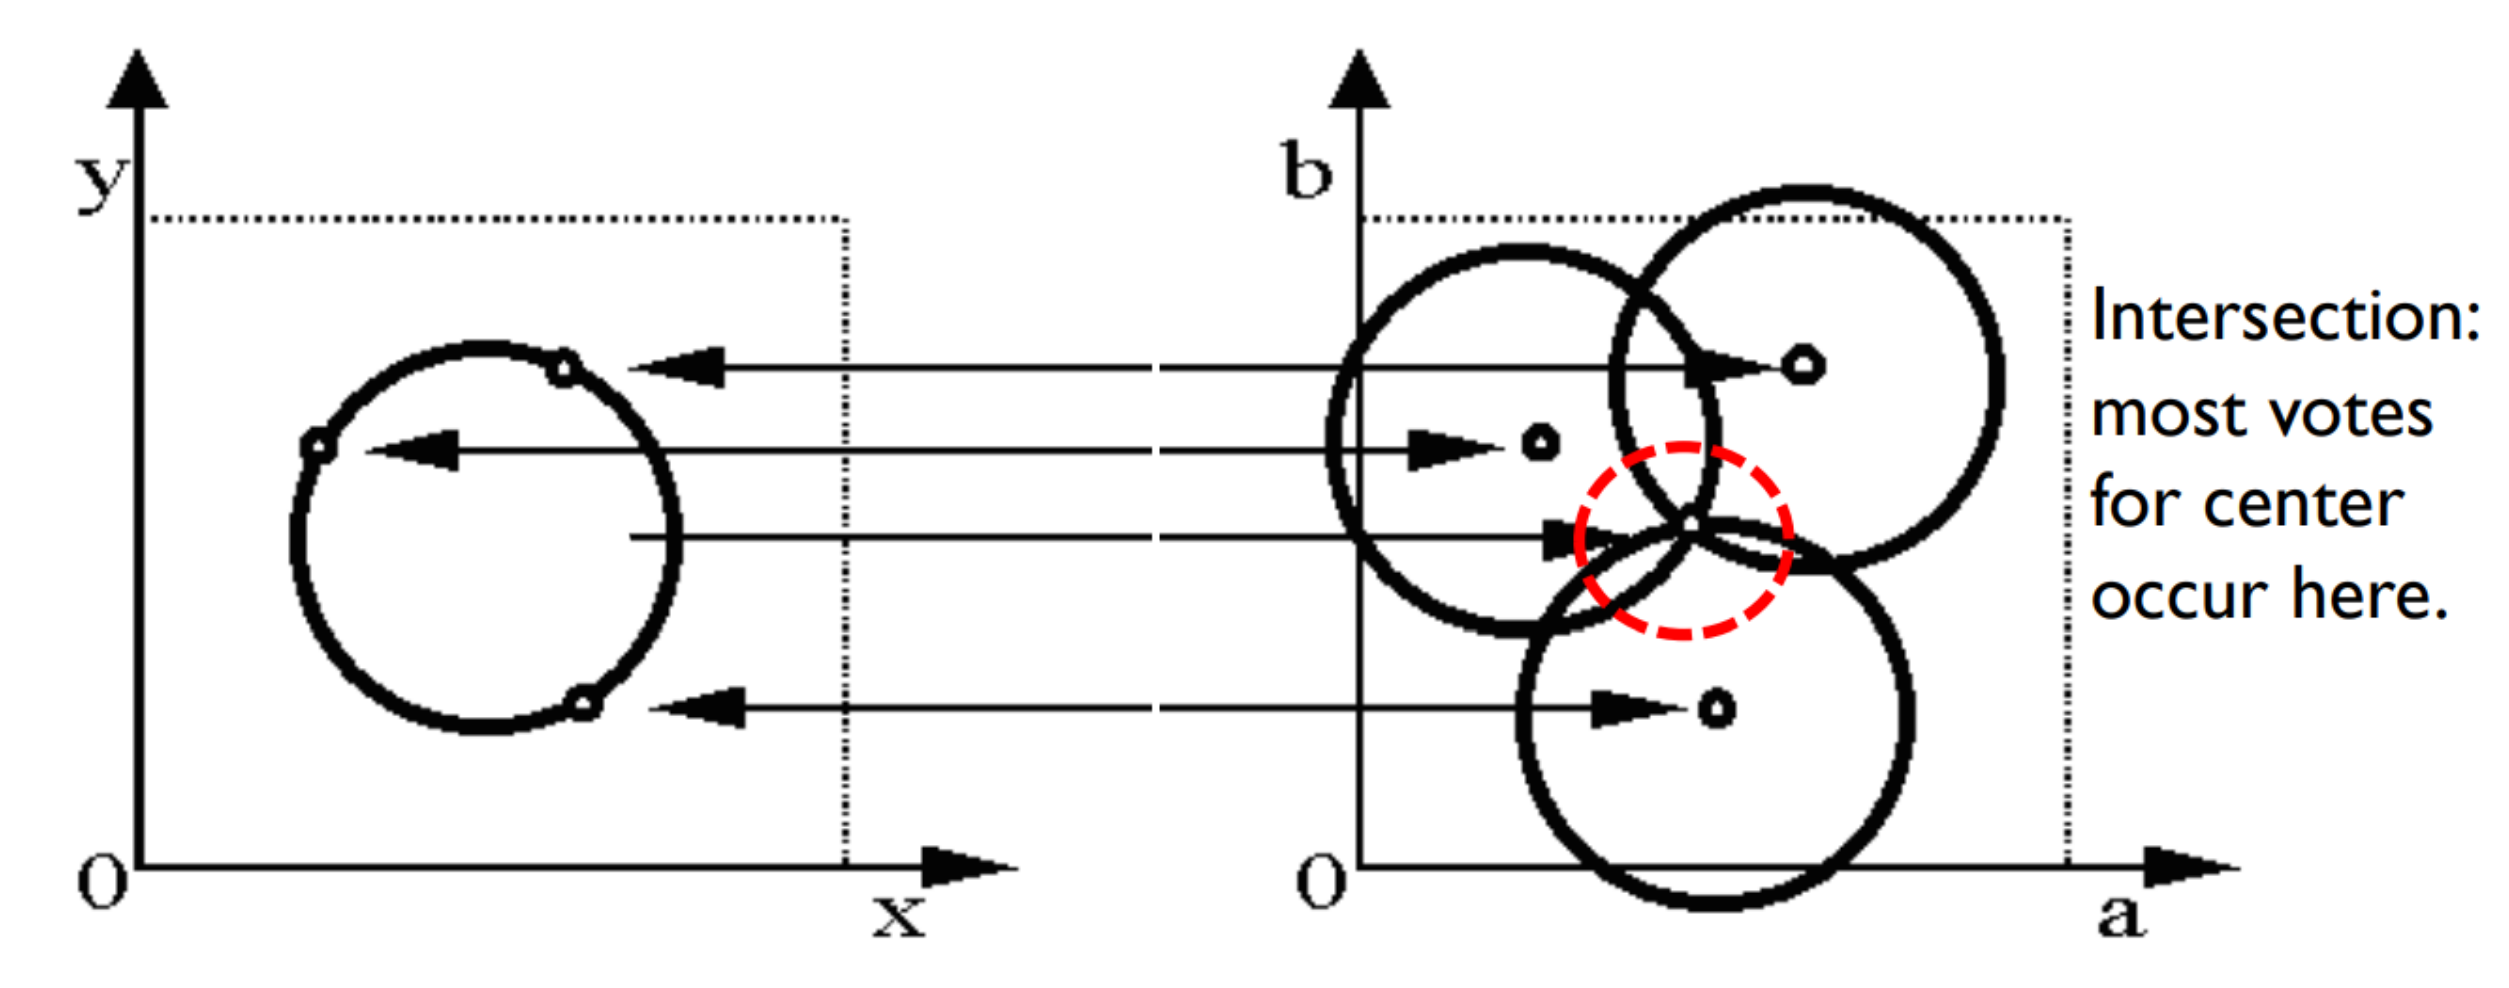
\includegraphics[width=0.7\linewidth]{img/hough_circle_accumulator}
\end{center}

\subsection{Hough Space for Circles With Unknown Radius}

\begin{center}
	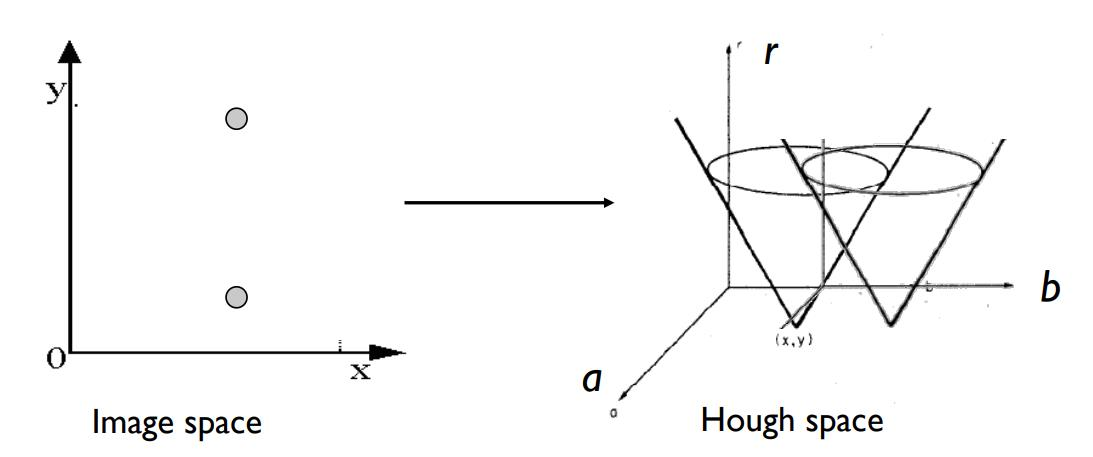
\includegraphics[width=0.7\linewidth]{img/hough_circle_accumulator_point}
\end{center}

\begin{equation*}
	y = a\cdot x + \sout{b}
\end{equation*}
